% intro/intro.tex

\chapter{Introduction}
\label{chp:Introduction}

\QuickQuizChapter{chp:Introduction}

Parallel programming has earned a reputation as one of the most
difficult areas a hacker can tackle.
Papers and textbooks warn of the perils of deadlock, livelock,
race conditions, non-determinism, Amdahl's-Law limits to scaling,
and excessive realtime latencies.
And these perils are quite real; we authors have accumulated uncounted
% 2008:
%	18 for Paul E. McKenney
years of experience dealing with them, and all of the emotional scars,
grey hairs, and hair loss that go with such an experience.

However, new technologies have always been difficult to use at introduction,
but have invariably become easier over time.
For example, there was a time when the ability to drive a car was a rare
skill, but in many developed countries, this skill is now commonplace.
This dramatic change came about for two basic reasons: (1) cars became
cheaper and more readily available, so that more people had the
opportunity to learn to drive, and (2) cars became simpler to operate,
due to automatic transmissions, automatic chokes, automatic starters,
improved reliability,
and a host of other technological improvements.

The same is true of a host of other technologies, including computers
themselves.
It is no longer necessary to operate a keypunch in order to program.
Spreadsheets allow most non-programmers to get results from their computers
that would have required a team of specialists a few decades ago.
Perhaps the most compelling example is web-surfing and content creation,
which since the early 2000s has been easily done by
untrained, uneducated people using various now-commonplace
social-networking tools.
As recently as 1968, such content creation was a far-out research
project~\cite{DouglasEngelbart1968}, described at
the time as
``like a UFO landing on the White House lawn''\cite{ScottGriffen2000}.
% http://www.ibiblio.org/pioneers/englebart.html
% http://www.histech.rwth-aachen.de/www/quellen/engelbart/ahi62index.html

Therefore, if you wish to argue that parallel programming will remain
as difficult as it is currently perceived by many to be, you must shoulder
the burden of proof, keeping in mind the many centuries of counter-examples
in a variety of fields of endeavor.

\section{Historic Parallel Programming Difficulties}
\label{sec:intro:Historic Parallel Programming Difficulties}

As indicated by its title, this book takes a different approach.
Rather than complain about the difficulty of parallel programming,
it instead examines the reasons why parallel programming is
difficult, and then works to help the reader to overcome these
difficulties.
As will be seen, these difficulties have fallen into several categories,
including:

\begin{enumerate}
\item	The historic high cost and relative rarity of parallel systems.
\item	The typical researcher's and practitioner's lack of experience
	with parallel systems.
\item	The paucity of publicly accessible parallel code.
\item	The lack of a widely understood engineering discipline of
	parallel programming.
\item	The high cost of communication relative to that of processing,
	even in tightly coupled shared-memory computers.
\end{enumerate}

Many of these historic difficulties are well on the way to being overcome.
First, over the past few decades, the cost of parallel systems
has decreased from many multiples of that of a house to a fraction of 
that of a used car, thanks to the advent of multicore systems.
Papers calling out the advantages of multicore CPUs were published
as early as 1996~\cite{Olukotun96}, IBM introduced simultaneous multi-threading
into its high-end POWER family in 2000, and multicore in 2001.
Intel introduced hyperthreading into its commodity Pentium line in
November 2000, and both AMD and Intel introduced
dual-core CPUs in 2005.
Sun followed with the multicore/multi-threaded Niagara in late 2005.
In fact, in 2008, it is becoming difficult
to find a single-CPU desktop system, with single-core CPUs being
relegated to netbooks and embedded devices.

Second, the advent of low-cost and readily available multicore system
means that the once-rare experience of parallel programming is
now available to almost all researchers and practitioners.
In fact, parallel systems are now well within the budget of students
and hobbyists.
We can therefore expect greatly increased levels of invention and
innovation surrounding parallel systems, and that increased familiarity
will over time make once-forbidding field of parallel programming
much more friendly and commonplace.

Third, where in the 20\textsuperscript{th} century, large systems of
highly parallel software were almost always closely guarded proprietary
secrets, the 21\textsuperscript{st} century has seen numerous
open-source (and thus publicly available) parallel software projects,
including the Linux kernel~\cite{Torvalds2.6kernel},
database systems~\cite{PostgreSQL2008,MySQL2008},
and message-passing systems~\cite{OpenMPI2008}.
This book will draw primarily from the Linux kernel, but will
provide much material suitable for user-level applications.

Fourth, even though the large-scale parallel-programming projects of
the 1980s and 1990s were almost all proprietary projects, these
projects have seeded the community with a cadre of developers who
understand the engineering discipline required to develop production-quality
parallel code.
A major purpose of this book is to present this engineering discipline.

Unfortunately, the fifth difficulty, the high cost of communication
relative to that of processing, remains largely in force.
Although this difficulty has been receiving increasing attention during
the new millenium, according to Stephen Hawkings,
the finite speed of light and the atomic
nature of matter is likely to limit progress in this
area~\cite{BryanGardiner2007,GordonMoore03a}.
Fortunately, this difficulty has been in force since the late 1980s,
so that the aforementioned engineering discipline has evolved practical
and effective strategies for handling it.
In addition, hardware designers are increasingly aware of these issues,
so perhaps future hardware will be more friendly to parallel software.
% @@@ discussed in chapter # @@@

\QuickQuiz{Come on now!!!
	Parallel programming has been known to be exceedingly
	hard for many decades.
	You seem to be hinting that it is not so hard.
	What sort of game are you playing?}
\QuickQuizAnswer{
	If you really believe that parallel programming is exceedingly
	hard, then you should have a ready answer to the question
	``Why is parallel programming hard?''
	One could list any number of reasons, ranging from deadlocks to
	race conditions to testing coverage, but the real answer is that
	{\em it is not really all that hard}.
	After all, if parallel programming was really so horribly difficult,
	how could a large number of open-source projects, ranging from Apache
	to MySQL to the Linux kernel, have managed to master it?

	A better question might be: ''Why is parallel programming {\em
	perceived} to be so difficult?''
	To see the answer, let's go back to the year 1991.
	Paul McKenney was walking across the parking lot to Sequent's
	benchmarking center carrying six dual-80486 Sequent Symmetry CPU
	boards, when he suddenly realized that he was carrying several
	times the price of the house he had just purchased.\footnote{
		Yes, this sudden realization {\em did} cause him to walk quite
		a bit more carefully.
		Why do you ask?}
	This high cost of parallel systems meant that
	parallel programming was restricted to a privileged few who
	worked for an employer who either manufactured or could afford to
	purchase machines costing upwards of \$100,000 --- in 1991 dollars US.

	In contrast, in 2006, Paul finds himself typing these words on a
	dual-core x86 laptop.
	Unlike the dual-80486 CPU boards, this laptop also contains
	2GB of main memory, a 60GB disk drive, a display, Ethernet,
	USB ports, wireless, and Bluetooth.
	And the laptop is more than an order of magnitude cheaper than
	even one of those dual-80486 CPU boards, even before taking inflation
	into account.

	Parallel systems have truly arrived.
	They are no longer the sole domain of a privileged few, but something
	available to almost everyone.

	The earlier restricted availability of parallel hardware is
	the \emph{real} reason that parallel programming is considered
	so difficult.
	After all, it is quite difficult to learn to program even the simplest
	machine if you have no access to it.
	Since the age of rare and expensive parallel machines is for the most
	part behind us, the age during which
	parallel programming is perceived to be mind-crushingly difficult is
	coming to a close.\footnote{
		Parallel programming is in some ways more difficult than
		sequential programming, for example, parallel validation
		is more difficult.
		But no longer mind-crushingly difficult.}
} \QuickQuizEnd

However, even though parallel programming might not be as hard as
is commonly advertised, it is often more work than sequential
programming.

\QuickQuiz{How could parallel programming \emph{ever} be as easy
	   as sequential programming???}
\QuickQuizAnswer{
	   It depends on the programming environment.
	   SQL~\cite{DIS9075SQL92} is an underappreciated success
	   story, as it permits programmers who know nothing about parallelism
	   to keep a large parallel system productively busy.
	   We can expect more variations on this theme as parallel
	   computers continue to become cheaper and more readily available.
	   For example, one possible contender in the scientific and
	   technical computing arena is MATLAB*P,
	   which is an attempt to automatically parallelize comon
	   matrix operations.
} \QuickQuizEnd

It therefore makes sense to consider alternatives to parallel programming.
However, it is not possible to reasonably consider parallel-programming
alternatives without understanding parallel-programming goals.
This topic is addressed in the next section.

\section{Parallel Programming Goals}
\label{sec:intro:Parallel Programming Goals}

@@@ Rewrite based on HOTPAR submission when published. @@@

What should your goals be when programming parallel systems?
Clearly, completing a correctly running program is always job 1.

But if performance is not a concern, you should instead do yourself
a favor and just write single-threaded code.
It will be easier, and you will probably get done much more quickly.

However, Moore's Law has ceased to provide its traditional performance
benefits, as can be seen in
Figure~\ref{fig:intro:Clock-Frequency Trend for Intel CPUs}.
This means that writing single-threaded code and simply waiting
a years or two for the CPUs to catch up may no longer be an option.
Given the recent trends on the part of all major manufacturers towards
multicore/multithreaded systems, parallelism is the way to go for
those wanting the avail themselves of the full performance of their
systems.

\begin{figure}[htb]
\begin{center}
\resizebox{3in}{!}{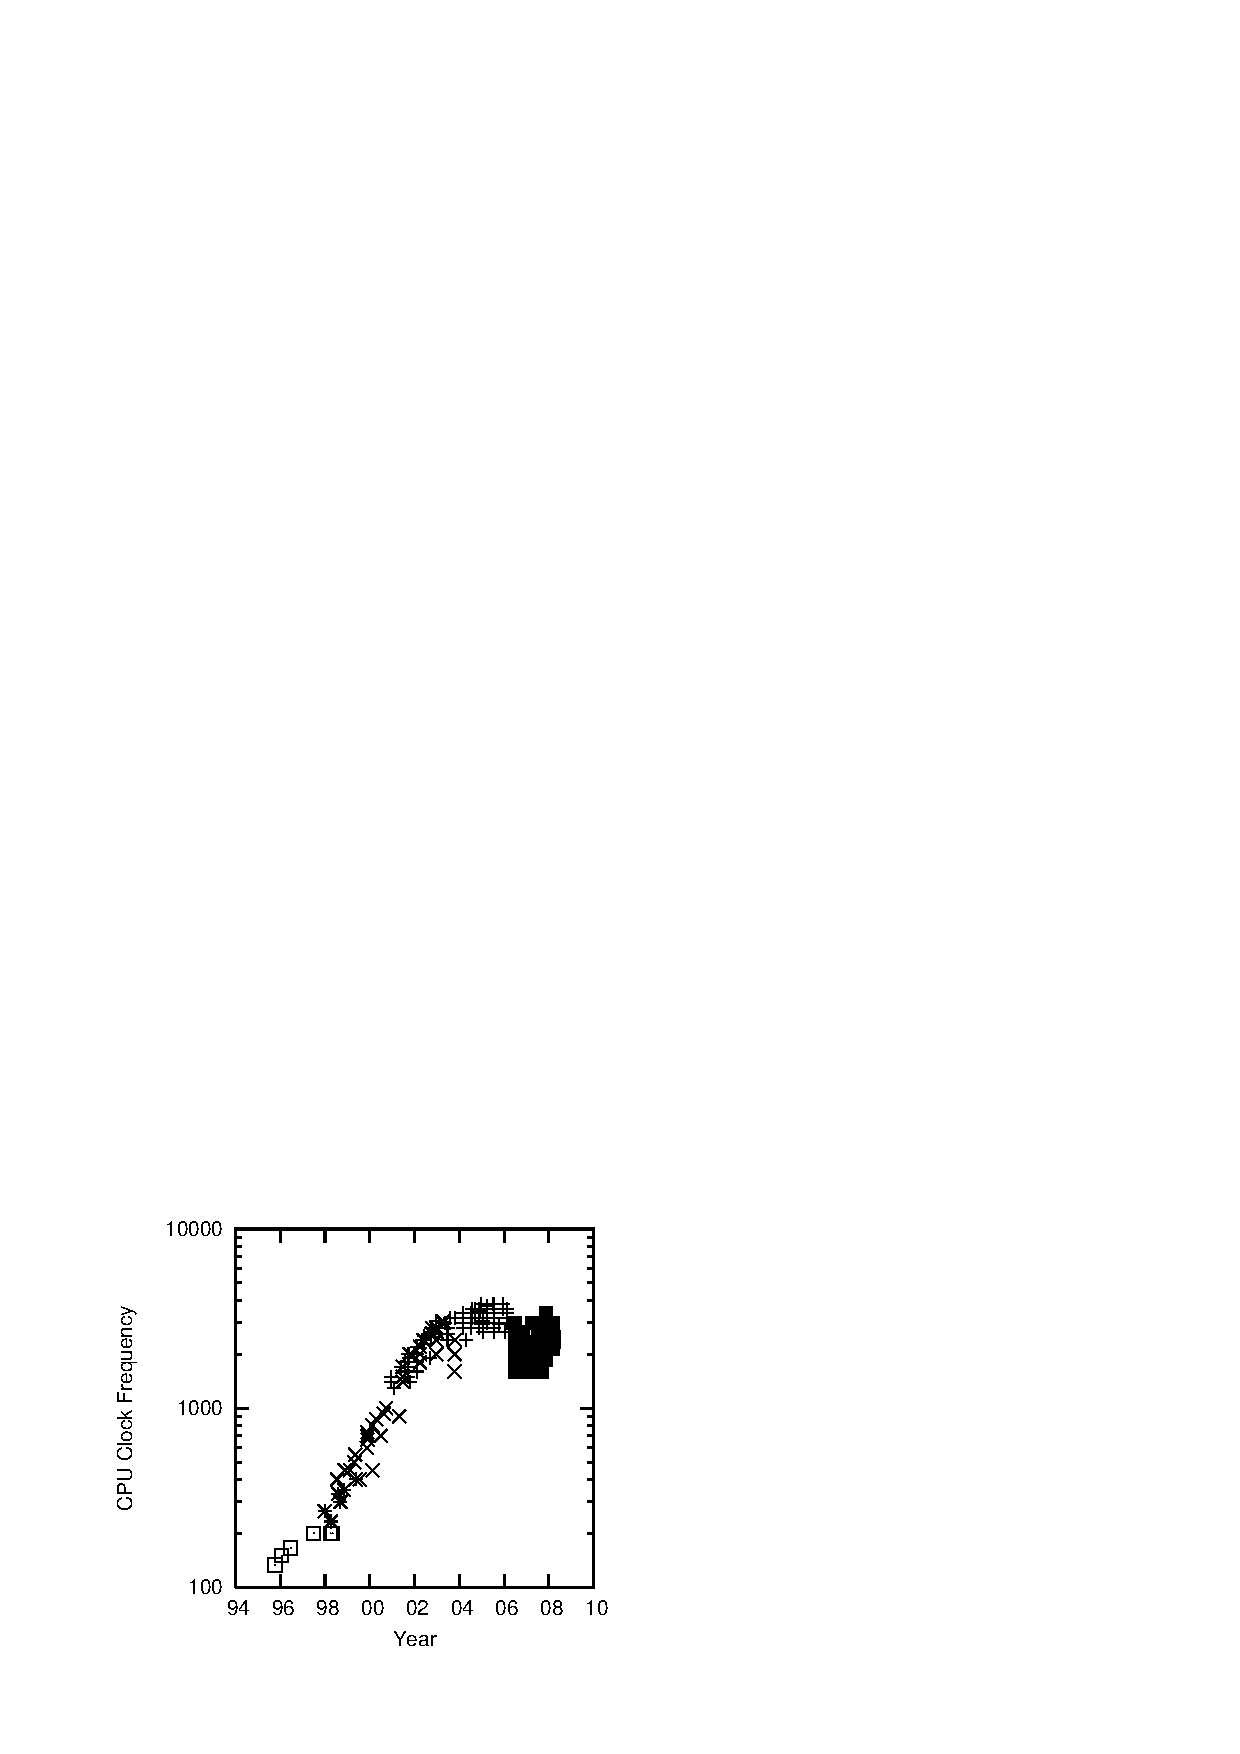
\includegraphics{SMPdesign/clockfreq}}
\end{center}
\caption{Clock-Frequency Trend for Intel CPUs}
\label{fig:intro:Clock-Frequency Trend for Intel CPUs}
\end{figure}

Even so, the first goal is performance rather than scalability,
especially given that the easiest way to attain linear scalability
is to reduce the performance of each CPU~\cite{LinusTorvalds2001a}.
Given a four-CPU system, which would you prefer?
A program that provides 100 transactions per second on a single CPU,
but does not scale at all?
Or a program that provides 10 transactions per second on a single CPU,
but scales perfectly?
The first program seems like a better bet, though the answer might
change if you happened to be one of the lucky few with access to a
32-CPU system.

Therefore, correctness first, performance second,
and scalability only as needed to
attain the required performance on whatever hardware your program
is to run on.

\section{Alternatives to Parallel Programming}
\label{sec:intro:Alternatives to Parallel Programming}

In order to properly consider alternatives to parallel programming,
you must first have thought through what you expect the parallelism
to do for you.
As seen in Section~\ref{sec:intro:Parallel Programming Goals},
typical goals include:

\begin{enumerate}
\item	Improve performance.
\item	Learn more about parallel programming.
\item	Have fun solving a parallel-programming problem.
\end{enumerate}

@@@ Adjust based on HOTPAR submission @@@

Although most developers might be most concerned with the first goal,
one advantage of the other goals is that they relieve you of the need
to justify using parallelism.
The remainder of this section is concerned only performance improvement.

It is important to keep in mind that parallelism is but one way to
improve performance.
Other well-known approaches include the following, in roughly increasing
order of difficulty:

\begin{enumerate}
\item	Run multiple instances of a sequential application.
\item	Construct the application to make use of existing parallel software.
\item	Apply performance optimization to the serial application.
\end{enumerate}

\subsection{Multiple Instances of a Sequential Application}
\label{sec:intro:Multiple Instances of a Sequential Application}

Running multiple instances of a sequential application can allow you
to do parallel programming without actually doing parallel programming.
There are a large number of ways to approach this, depending on the
structure of the application.

If your program is analyzing a large number of different scenarios,
or is analyzing a large number of independent data sets, one easy
and effective approach is to create a single sequential program that
carries out a single analysis, then use any of a number of scripting
enviroments (for example the \url{bash} shell) to run a number of
instances of this sequential program in parallel.
In some cases, this approach can be easily extended to a cluster of
machines.

This approach may seem like cheating, and in fact some denigrate such
programs ``embarrassingly parallel''.
And in fact, this approach does have some potential disadvantages,
including increased memory consumption, waste of CPU cycles recomputing
common intermediate results, and increased copying of data.
However, it is often  extremely effective, garnering extreme performance
gains with little or no added effort.

\subsection{Make Use of Existing Parallel Software}
\label{sec:intro:Make Use of Existing Parallel Software}

There is no longer any shortage of parallel software environments that
can present a single-threaded programming environment,
including relational
databases, web-application servers, and map-reduce environments.
For example, a common design provides a separate program for each
user, each of which generates SQL that is run against a common
relational database.
The per-user programs are responsible only for the user interface,
wiht hte relational database taking full responsbility for the
difficult issues surrounding parallelism and persistence.

\subsection{Performance Optimization}
\label{sec:intro:Performance Optimization}

Up through the early 2000s, CPU performance was doubling every 18 months.
In such an environment, it is often much more important to create new
functionality than to do careful performance optimization.
Now that Moore's Law is ``only'' increasing transistor density instead
of increasing both transistor density and per-transistor performance,
it might be a good time to rethink the importance of performance
optimization.

After all, performance optimization can reduce power consumption as
well as increasing performance.

Performance analysis of sequential programs is well understood,
and will not be discussed further here.
Instead, we will look at parallel programming as yet another performance
optimization, albeit one that has recently become very important due
to the widespread availability of low-cost multicore systems.

\section{Ease of Use}
\label{sec:intro:Ease of Use}

We are talking about parallel performance and latency,
so why is ease of use important?

Because the easier a performance technique is to use, the more likely
it will be used.
This greater use can outweigh a small performance penalty compared
to an optimal hard-to-use technique.

This book is not a collection of optimal algorithms with tiny areas of
applicability; instead, it is a handbook of widely applicable and heavily
used techniques.
We of course could not resist the urge to include some of our favorites
that have not (yet!) passed the test of time (what author could?), but
we have nonetheless gritted our teeth and banished our darlings to
appendices.
Perhaps in time, some of them will see enough use that we can promote
them into the main body of the text.

\section{Guide to This Book}
\label{sec:intro:Guide to This Book}

\emph{@@@ More here.  Sections.  Layered Approach.  Appendices.
Quick Quizzes.  Glossary.  Bibliography.}

\subsection{Quick Quizzes}

``Quick quizzes'' appear throughout this book.
Some of these quizzes are based on material in which that quick quiz
appears, but others require you to think beyond that section, and,
in some cases, beyond the entire book.
As with most endeavors, what you get out of this book is largely
determined by what you are willing to put into it.
Therefore, readers who invest some time into these quizzes will
find their effort repaid handsomely with increased understanding
of parallel programming.

Answers to the quizzes may be found
in
Appendix~\ref{chp:Answers to Quick Quizzes} starting on
page~\pageref{chp:Answers to Quick Quizzes}.

\QuickQuiz{Where are the answers to the Quick Quizzes found?}
\QuickQuizAnswer{
	In Appendix~\ref{chp:Answers to Quick Quizzes} starting on
	page~\pageref{chp:Answers to Quick Quizzes}.

	Hey, I thought I owed you an easy one!!!
} \QuickQuizEnd

\QuickQuiz{Some of the Quick Quiz questions seem to be from the viewpoint
	of the reader rather than the author.
	Is that really the intent?}
\QuickQuizAnswer{
	Indeed it is!
 	Many are modeled after Paul (just ask anyone who has had the
	misfortune of being assigned to teach him).
	Others are quite similar to actual questions that have been asked
	during conference presentations and lectures covering the
	material in this book.
	Still others are from the viewpoint of the author.
} \QuickQuizEnd

\subsection{Sample Source Code}

This book discusses its fair share of source code, and in many cases
this source code may be found in the \url{CodeSamples} directory
of this book's git tree.
For example, on UNIX systems, you should be able to type:
\begin{verbatim}
	find CodeSamples -name rcu_rcpls.c -print
\end{verbatim}
to locate the file \url{rcu_rcpls.c}, which is called out in
Section~\ref{defer:``Toy'' RCU Implementations}.
Other types of systems have well-known ways of locating files by
filename.

The source to this book may be found in the \url{git} archive at
\url{git://git.kernel.org/pub/scm/linux/kernel/git/paulmck/perfbook.git},
and \url{git} itself is available as part of most mainstream Linux
distributions.
